% ****** Start of file aipsamp.tex ******
%
%   This file is part of the AIP files in the AIP distribution for REVTeX 4.
%   Version 4.1 of REVTeX, October 2009
%
%   Copyright (c) 2009 American Institute of Physics.
%
%   See the AIP README file for restrictions and more information.
%
% TeX'ing this file requires that you have AMS-LaTeX 2.0 installed
% as well as the rest of the prerequisites for REVTeX 4.1
% 
% It also requires running BibTeX. The commands are as follows:
%
%  1)  latex  aipsamp
%  2)  bibtex aipsamp
%  3)  latex  aipsamp
%  4)  latex  aipsamp
%
% Use this file as a source of example code for your aip document.
% Use the file aiptemplate.tex as a template for your document.
\documentclass[%
 aps,
% jmp,
% bmf,
% sd,
% rsi,
 amsmath,amssymb,
preprint,%
%reprint,%
superscriptaddress,
%author-year,%
%author-numerical,%
% Conference Proceedings
]{revtex4-2}

\usepackage{graphicx}% Include figure files
\graphicspath{{NewFigures/}}
\usepackage{dcolumn}% Align table columns on decimal point
\usepackage{bm}% bold math
%\usepackage[mathlines]{lineno}% Enable numbering of text and display math
%\linenumbers\relax % Commence numbering lines

\usepackage[utf8]{inputenc}
\usepackage[T1]{fontenc}
\usepackage{mathptmx}
\usepackage{xcolor}
\usepackage{epstopdf}
\usepackage{floatrow}
\usepackage{hyperref}
% \usepackage{caption}
% \usepackage[justification=justified, format=plain]{caption}
\hypersetup{
  colorlinks   = true, %Colours links instead of ugly boxes
  urlcolor     = blue, %Colour for external hyperlinks
  linkcolor    = blue, %Colour of internal links
  citecolor   = blue %Colour of citations
}

\begin{document}
\renewcommand{\theequation}{S\arabic{equation}}

% \renewcommand{\thepage}{S\arabic{page}} 
% \renewcommand{\thesection}{S\arabic{section}}  
\renewcommand{\thetable}{S\arabic{table}}  
\renewcommand{\thefigure}{S\arabic{figure}} 


\preprint{APS/123-QED}

\title[]{\underline{Supplemental material} \\ Dynamics of coupled thermoacoustic oscillators\\ under asymmetric forcing: Experiments and {\color{blue}theoretical modeling}}

%\author[2]{Premchand C P}
%\author[1]{Manikandan Raghunathan}
%\author[1]{Abin Krishnan}
%\author[2]{Vineeth Nair}
%\author[1]{Sujith R I}
%\address[1]{Department of Aerospace Engineering, IIT Madras, Tamil Nadu - 600 036, India}
%\address[2]{Department of Aerospace Engineering, IIT Bombay, Maharashtra - 400 076, India}

\author{Ankit Sahay}
 \email[Corresponding Author: ]{ankitsahay02@gmail.com}
 \affiliation{Department of Aerospace Engineering, IIT Madras, Tamil Nadu - 600 036, India} 
\author{Amitesh Roy}
\affiliation{Department of Aerospace Engineering, IIT Madras, Tamil Nadu - 600 036, India}

\author{Samadhan A. Pawar}
\affiliation{Department of Aerospace Engineering, IIT Madras, Tamil Nadu - 600 036, India} 

\author{R I Sujith}
\affiliation{Department of Aerospace Engineering, IIT Madras, Tamil Nadu - 600 036, India} 

\date{\today}% It is always \today, today,

\maketitle

%\begin{quotation}
%This is the lead paragraph.
%\end{quotation}

\section{\label{R_square} $R^2$ values for synchronization boundaries}

\begin{table}[h]
\caption{\label{tab:table1} $R^2$ values of least-square-fitted boundaries of the Arnold tongue. The subscripts $l,r$ denote the left and right boundaries, respectively.}
\begin{ruledtabular}
\begin{tabular}{cccccc}
 & & \multicolumn{2}{c}{Rijke tube A}&\multicolumn{2}{c}{Rijke tube B}\\
 Figures & $p^\prime_{0}$ & $R^2_l$ & $R^2_r$ & $R^2_l$ & $R^2_r$ \\ \hline
 Fig. 2 & 120 Pa & 0.98 & 0.96 & - & - \\
        & 200 Pa & 0.96 & 0.85 & - & - \\
 Fig. 6 & 120 Pa & 0.99 & 0.88 & 0.96 & 1.00 \\
        & 200 Pa & 0.95 & 0.89 & 0.94 & 0.81 \\
 Fig. 7 & 120 Pa & 0.98 & 0.93 & 0.94 &  -   \\
        & 200 Pa & 0.97 & 0.99 &   -  &  -   \\
     \textcolor{blue}{Fig. 8} &        & \textcolor{blue}{0.98} & \textcolor{blue}{0.98} &  \textcolor{blue}{-} & \textcolor{blue}{-} \\
 \textcolor{blue}{Fig. 11} &       & \textcolor{blue}{0.91} & \textcolor{blue}{0.98} & \textcolor{blue}{0.98} & \textcolor{blue}{0.99} \\
 \textcolor{blue}{Fig. 12} &       & \textcolor{blue}{0.98} & \textcolor{blue}{0.98} & \textcolor{blue}{-} & \textcolor{blue}{0.98} \\
\end{tabular}
\end{ruledtabular}
\end{table}

Table \ref{tab:table1} shows the $R^2$ values obtained when a linear fit is applied to the data points on the forced synchronization boundaries in the $\bar{A}_f-f_f$ plane. Figures 2, 6 and 7 refer to experimental results shown in the main manuscript, whereas Figs. 8, 11 and 12 refer to results obtained from the mathematical model. An $R^2 = 1$ indicates that the linear regression predictions perfectly fit the data. 

\newpage

\section{Period-3 oscillations exhibit by a single Rijke tube oscillator under external forcing}
\label{Period_3}

\begin{figure*}[h!]
\centering
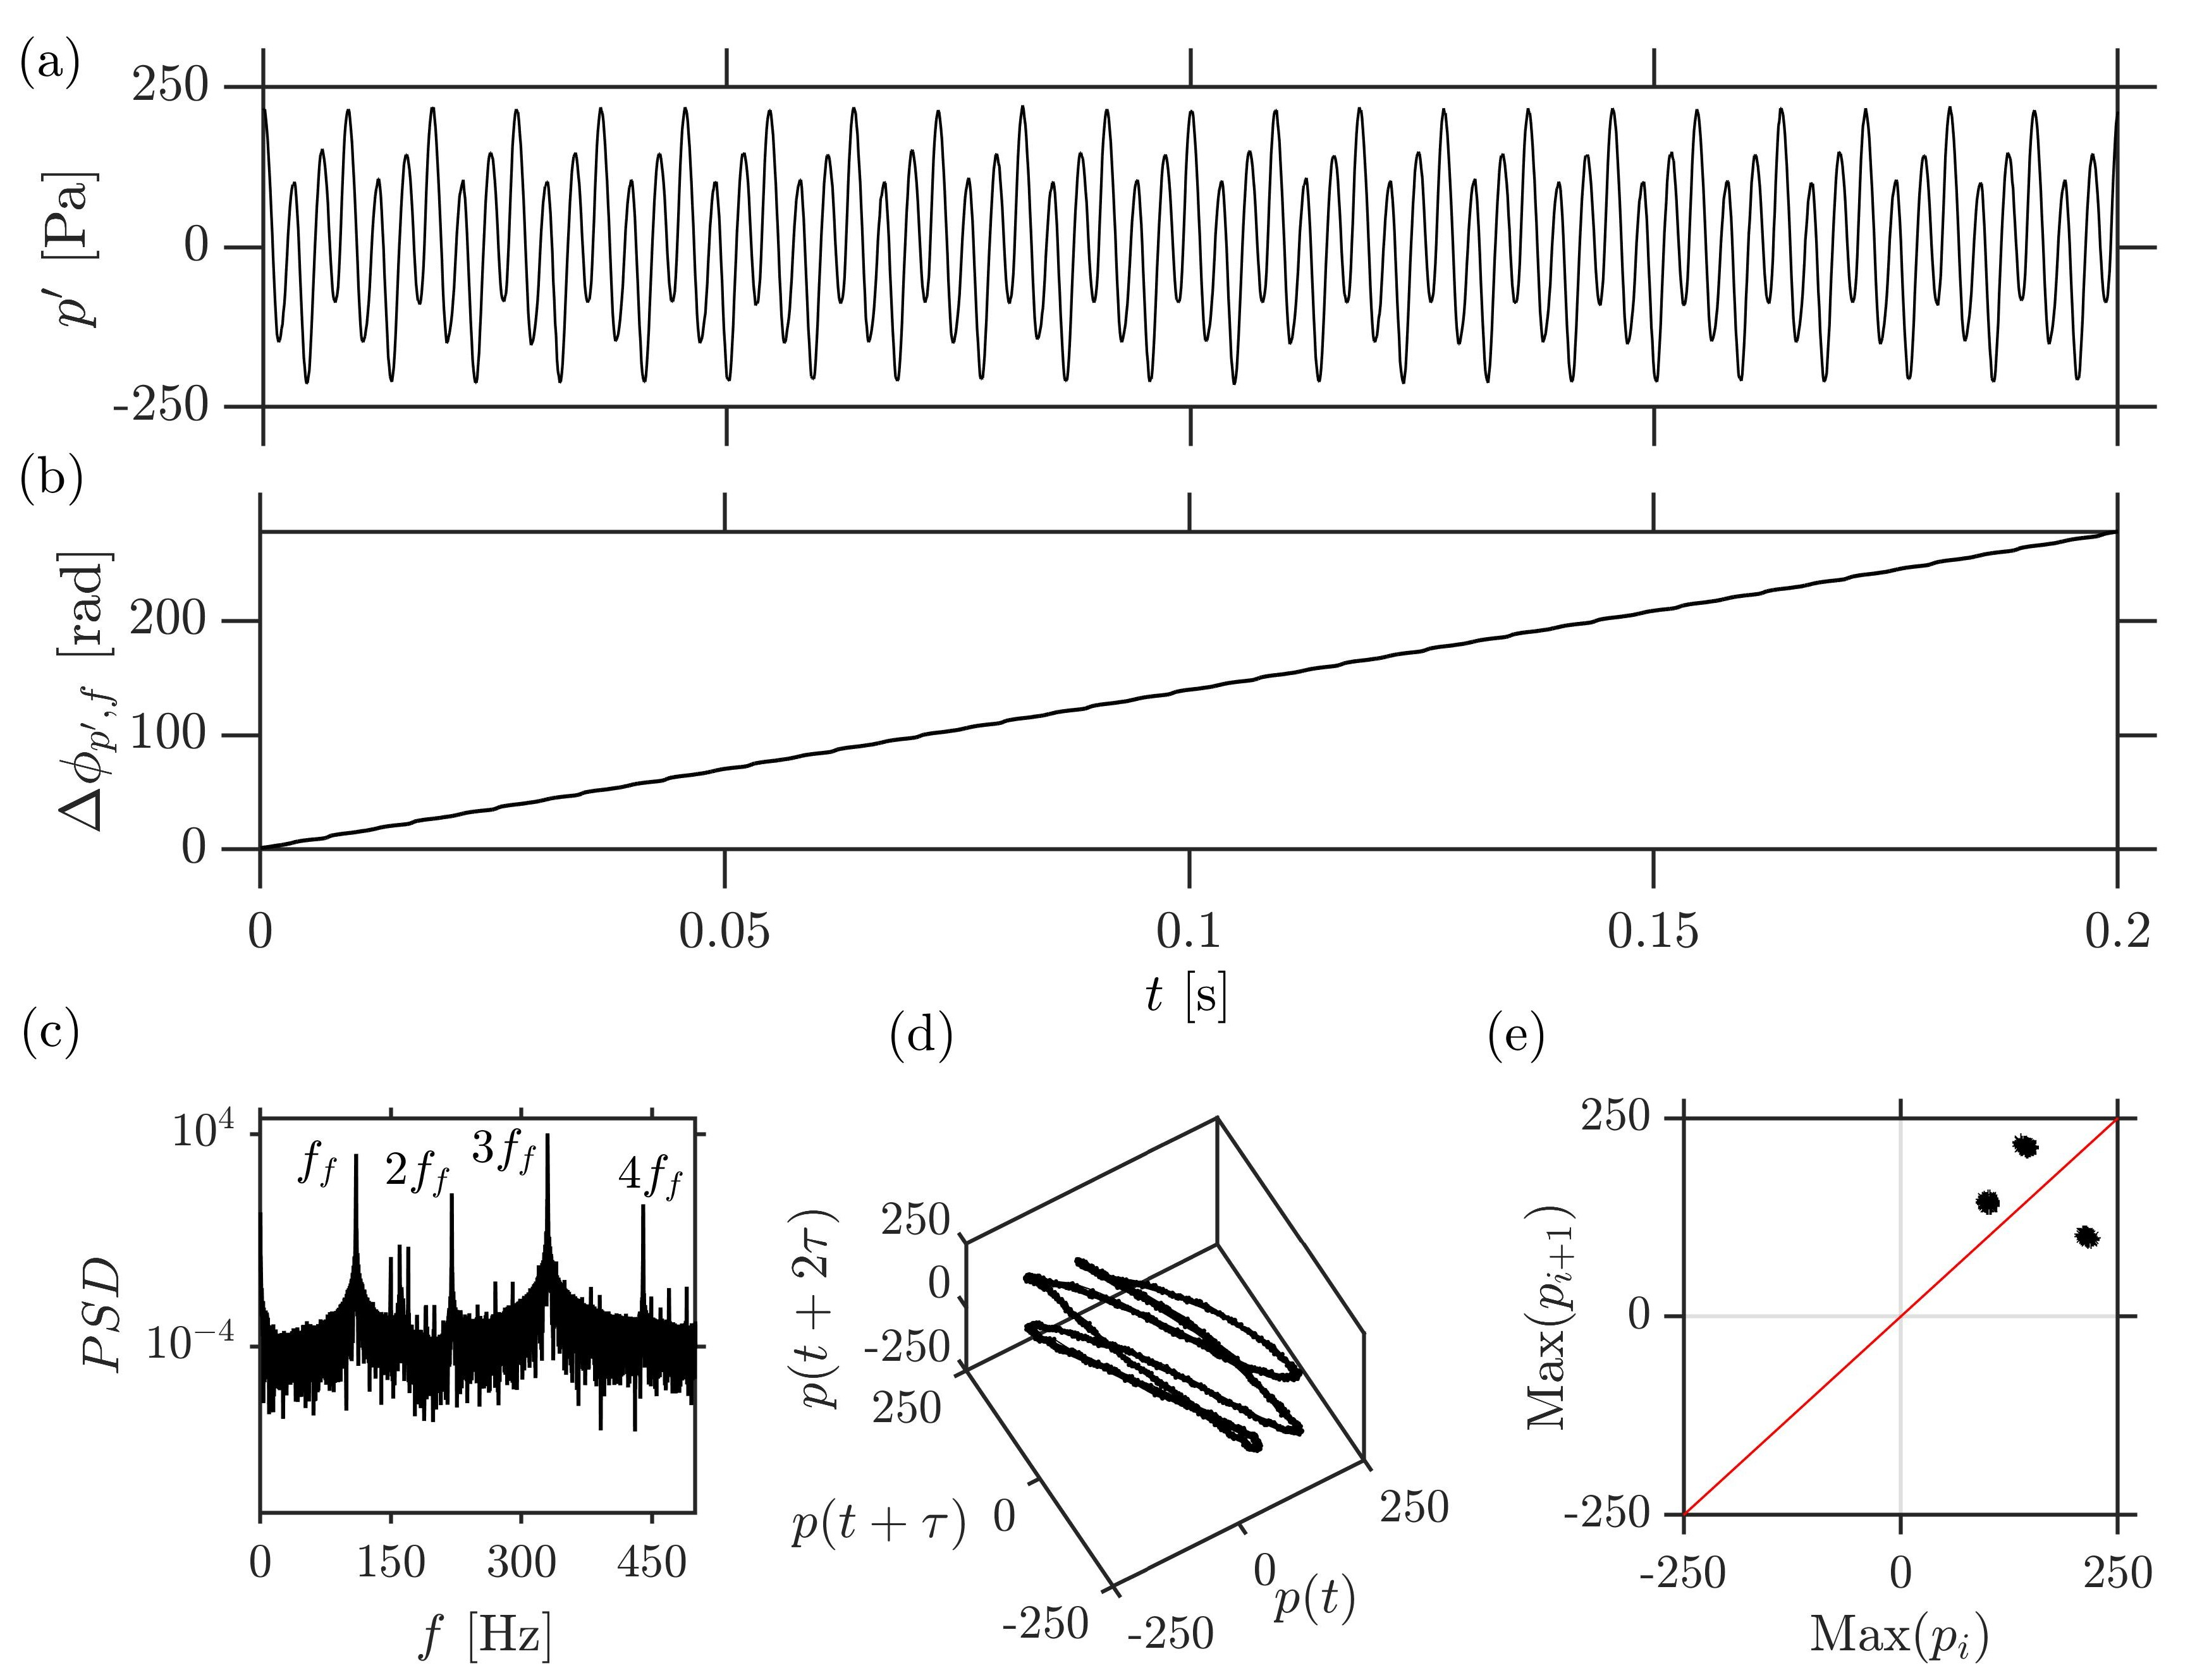
\includegraphics[scale=0.13]{fig8_single_osc_110Hz_28mV_200Pa_LCO.jpg}
\caption{\label{superharmonic} Time series of (a) the acoustic pressure fluctuations and (b) instantaneous phase difference between the pressure and the forcing signal. (c) The power spectrum, (d) the reconstructed phase portrait, and (e) the first return map of the forced acoustic pressure oscillations in a single Rijke tube exhibiting LCO of amplitude $p^\prime_{0} = 200$ Pa. The forcing is applied at $f_f/f_{n0} = 0.69$ and $\bar{A}_f= 0.65$. As a result, the acoustic pressure fluctuations show period-3 oscillations and, hence, remain desynchronized with the forcing signal, causing a lower value of \textit{PLV}. The period-3 oscillations are confirmed from the presence of three-looped attractor in the phase space and three fixed points in the return map.} 
\end{figure*}

During experiments in a single Rijke tube oscillator, we observe period-3 behavior in $p^\prime$ for high values of $\bar{A}_f$ in $f_f/f_{n0} = 0.62-0.70$ range, which leads to low $PLV$ calculated between the $p^\prime$ and forcing signal. In Fig. \ref{superharmonic}a, we show the acoustic pressure fluctuations exhibited by the Rijke tube at $f_f/f_{n0} = 0.69$ and $\bar{A}_f = 0.65$. The unforced amplitude of the LCO exhibited by the Rijke tube is $p^\prime_{0} = 200$ Pa. The period-3 behavior can be observed from the time series in Fig. \ref{superharmonic}a, as well as the spectral peaks in Fig. \ref{superharmonic}c, where we notice the presence of spectral peaks of approximately same magnitude at $f_f, 2f_f$ and $3f_f$ locations. Correspondingly, in Fig. \ref{superharmonic}d, the structure representative of the system dynamics (referred to hereinafter as the attractor) is a triple-looped attractor, i.e., the trajectories need to loop thrice before coming back to the initial point. Because the orbit is periodic, we get three distinct dots in the single-sided return map for the acoustic pressure time series in Fig. \ref{superharmonic}e.

\newpage

\textcolor{blue}{\section{ Effect of varying coupling tube parameters on the amplitude dynamics of an identical Rijke tubes coupled system}}
\label{Supp_mat_3}

\begin{figure*}[h!]
\centering
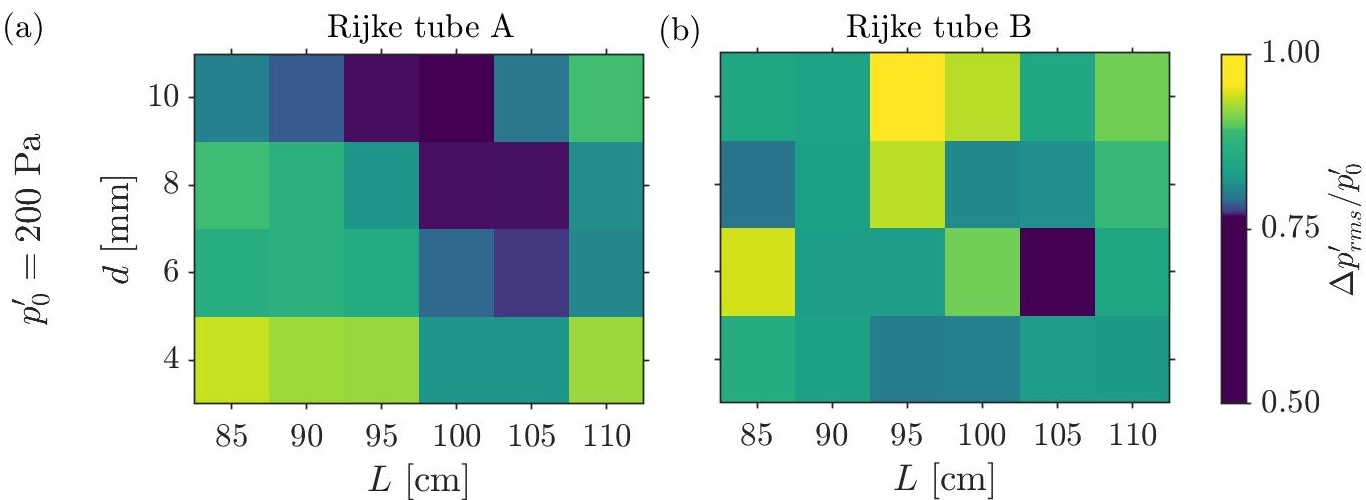
\includegraphics[scale=0.45]{d_vs_l_prms.jpg}
\caption{\label{d_vs_l}Experimental two-parameter bifurcation plots showing the variation of $\Delta p^\prime_{rms}/p^\prime_{0}$ for different values of coupling tube length $L$ and internal diameter $d$ in identical Rijke tubes ($\Delta f_{n0} = 0$ Hz). The maximum suppression obtained is around 50\% in Rijke tube A for $L =100$ cm and $d =10$ mm.} 
\end{figure*}

Here, we explore experimentally the suppression of LCO in coupled Rijke tubes for connecting tubes of varying lengths and internal diameters. Figure \ref{d_vs_l} shows the reduction in the amplitude of LCO for different combinations of $L$ and $d$ for identical Rijke tubes. We notice that for $d=10$ mm, we obtain maximum suppression of about 50\% in the acoustic pressure fluctuations for $L \sim 100$ cm, in Rijke tube A. Thus, we keep $d=10$ mm for all our experiments. Large diameter connecting tubes may not be feasible for real-time combustors as it will require significant modification to engine hardware, whereas smaller diameters of connecting tube, such as the one used in the present study, can be very easily implemented.

\newpage

% \begin{figure*}[t!]
% \centering
% \includegraphics[scale=0.43]{K_vs_tau_tube.jpg}
% \caption{\label{K_vs_tau} Two-parameter bifurcation plots in $K-\tau_{tube}$ plane, demarcating the regions of AD and LCO in a system of coupled identical Rijke tube oscillators. (a) $K_d$ is increased as $0.0$, $0.1$ and $1.0$ while keeping $K_{\tau}$ fixed at $0.5$. (b) $K_{\tau}$ is increased as $0.1$, $0.3$ and $0.5$ while keeping $K_{d}$ fixed at $1.0$. The region of AD increases in size with increase in the value of $K_d$ and $K_{\tau}$. For $K_d = 0.0$ and $0.1$, the region of AD is centered around odd multiples of $\tau_{tube}=0.45$. For larger values of $K_d$, the region of AD appears centered around odd multiples of $\tau_{tube}=0.9$. Such a recurrence of AD at odd multiples of some optimum $\tau_{tube}$ has been reported previously in \citet{hyodo2018stabilization}}
% \end{figure*}

% Figure \ref{K_vs_tau} shows the effect of time-delay and dissipative couplings on the region of amplitude death (AD) obtained from the coupled Rijke tube model given in Eqs. (\ref{eq:13}) and (\ref{eq:14}). The two coupled oscillators are kept identical. In Fig. \ref{K_vs_tau}, we observe that as the value of coupling constants increase, the region of AD increases in size. This behavior is consistent when either of the coupling parameters ($K_d$ and $K_{\tau}$) is kept constant, and the other one is increased. We also note that the region of AD is quite limited when dissipative or time-delay coupling are applied individually, as also noted in \cite{thomas2018effect}. Thus, it becomes easier to achieve amplitude death when the magnitudes of coupling parameters are increased. Further, in Fig. \ref{K_vs_tau}a, we observe that for $K_d = 0.0$ and $0.1$, the region of AD is centered around odd multiples of $\tau_{tube}=0.45$. For larger values of $K_d$, the region of AD appears centered around odd multiples of $\tau_{tube}=0.9$. Such a recurrence of AD at odd multiples of some optimum $\tau_{tube}$ has been reported previously in \citet{hyodo2018stabilization}.

\textcolor{blue}{\section{ Mathematical model}}
\label{model}

Here, we derive a reduced-order model for the coupled horizontal Rijke tubes subjected to asymmetric forcing. The model is based on \citet{balasubramanian2008thermoacoustic}. We neglect the effects of mean flow and mean temperature gradient in the duct. For two Rijke tubes A \& B, the acoustic momentum and energy equations for a medium with a perfect, inviscid and non-heat conducting gas are then given as \cite{balasubramanian2008thermoacoustic}:
\begin{equation} \label{eq:1}
    \bar{\rho}\dfrac{\partial \Tilde{u_a}^\prime}{\partial \Tilde{t}} + \dfrac{\partial \Tilde{p_a}^\prime}{\partial \Tilde{x}} = 0,
\end{equation}

\begin{equation} \label{eq:2}
    \dfrac{\partial \Tilde{p_a}^\prime}{\partial \Tilde{t}} + \gamma \bar{p}\dfrac{\partial \Tilde{u_a}^\prime}{\partial \Tilde{x}} = (\gamma -1)\Dot{\Tilde{Q}}^\prime \delta(\Tilde{x}-\Tilde{x_f}),
\end{equation}

\begin{equation} \label{eq:3}
    \bar{\rho}\dfrac{\partial \Tilde{u_b}^\prime}{\partial \Tilde{t}} + \dfrac{\partial \Tilde{p_b}^\prime}{\partial \Tilde{x}} = 0,
\end{equation}

\begin{equation} \label{eq:4}
    \dfrac{\partial \Tilde{p_b}^\prime}{\partial \Tilde{t}} + \gamma \bar{p}\dfrac{\partial \Tilde{u_b}^\prime}{\partial \Tilde{x}} = (\gamma -1)\Dot{\Tilde{Q}}^\prime \delta(\Tilde{x}-\Tilde{x_f}).
\end{equation}


where, $\Tilde{p}^\prime$ and $\Tilde{u}^\prime$ are the acoustic pressure and velocity fluctuations, respectively. $\gamma$ is the ratio of specific heats of air at ambient conditions. $\Tilde{x}$ is the distance along the axial direction in the duct, $\Tilde{t}$ is the time, $\bar{\rho}$ and $\bar{p}$ are the ambient density and pressure, respectively. Subscripts $a$ and $b$ indicate the quantities correpsonding to Rijke tube A \& B, respectively. For a general system of non-identical oscillators, we define a quantity $r$ as:
\begin{equation} \label{eq:5}
r = \dfrac{L_b}{L_a} = \dfrac{\omega_b}{\omega_a},
\end{equation}
where, $L_a$ and $L_b$ are lengths of the Rije tube ducts A \& B, respectively. $\omega_a$ and $\omega_b$ are the natural frequencies of the Rijke tubes A and B, respectively.

We non-dimensionalize Eqs. (\ref{eq:1}) and (\ref{eq:4}) using the following transformations:
\begin{equation} \label{eq:6}
    x = \dfrac{\Tilde{x}}{L_a}; \hspace{5 pt} t = \dfrac{c_0}{L_a}\Tilde{t}; \hspace{5 pt} u_{a}^\prime = \dfrac{\Tilde{u_a}^\prime}{u_0}; \hspace{5 pt} p_{a}^\prime = \dfrac{\Tilde{p_a}^\prime}{\bar{p}}; \hspace{5 pt} M = \dfrac{u_0}{c_0}; \hspace{5 pt} u_{b}^\prime = \dfrac{\Tilde{u_b}^\prime}{u_0}; \hspace{5 pt} p_{b}^\prime = \dfrac{\Tilde{p_b}^\prime}{\bar{p}}; \hspace{5 pt} \Dot{Q}^\prime = \dfrac{\Dot{\Tilde{Q}}^\prime}{c_0 \bar{p}}.
\end{equation}
Here, variables with tilde are dimensional and variables without tilde are non-dimensional. $u_0$ and $\bar{p}$ are the steady state velocity and pressure of the flow, respectively. $c_0$ is the speed of sound, and $M$ is the Mach number of the mean flow. $x$ and $t$ are the non-dimensional axial distance and time, respectively. Using the above transformations, we obtain the following non-dimensionlized acoustic momentum and energy equations:
\begin{equation} \label{eq:7}
    \gamma M \dfrac{\partial u_a^\prime}{\partial t} + \dfrac{\partial p_a^\prime}{\partial x} = 0,
\end{equation}

\begin{equation} \label{eq:8}
    \dfrac{\partial p_a^\prime}{\partial t} + \gamma M \dfrac{\partial u_a^\prime}{\partial x} = \dfrac{(\gamma -1)L_a \Dot{Q}^\prime}{\bar{p}c_0} \delta[L_a(x-x_f)],
\end{equation}

\begin{equation} \label{eq:9}
\gamma M \dfrac{\partial u_b^\prime}{\partial t} + \dfrac{\partial p_b^\prime}{\partial x} = 0,
\end{equation}

\begin{equation} \label{eq:10}
\dfrac{\partial p_b^\prime}{\partial t} + \gamma M \dfrac{\partial u_b^\prime}{\partial x} = \dfrac{(\gamma -1)L_a \Dot{Q}^\prime}{\bar{p}c_0} \delta[L_a(x-x_f)].
\end{equation}

The heat release rate $\Dot{Q}^\prime$ is modeled using a modified form of King's law \cite{king1914xii, heckl1990non} which correlates the quasi-steady heat transfer from a heated cylinder to the flow around it. The expression for normalized heat release rate fluctuations is written in terms of the acoustic velocity fluctuations, observed at the heater location $x_f$ after time delay $\tau$ as:
\begin{equation} \label{eq:11}
    \Dot{Q}^\prime = \dfrac{2L_{w}(T_{w}-\bar{T})}{S\sqrt{3}} \sqrt{\pi \lambda C_{v}\bar{\rho} \dfrac{d_w}{2}}
 \left[  \sqrt{\left| \dfrac{u_0}{3} + u_{f}^\prime(t-\tau) \right|}-\sqrt{\dfrac{u_0}{3}}\right],
\end{equation} where, $d_w$, $L_w$ and $T_w$ are the diameter, length and temperature of the heater wire, respectively. $\bar{T}$ is the steady state temperature of the flow, $S$ is the cross-sectional area of the duct, $C_v$ \& $\lambda$ are the specific heat at constant volume and thermal conductivity, respectively, of the medium within the duct. $\tau$ quantifies the thermal inertia of the heat transfer from the heating element to the medium.

The non-dimensionalized set of PDEs in Eqs. (\ref{eq:7})-(\ref{eq:10}) is reduced to a set of ordinary differential equations using the Galerkin technique \cite{lores1973nonlinear}. To that end, the non-dimensional velocity $u^\prime$ and non-dimensional pressure $p^\prime$ fluctuations in the model are written in terms of the Galerkin modes:

\begin{equation} \label{eq:12}
    p_a^\prime(x,t) =  \sum_{j=1}^{N} -\dfrac{\gamma M}{j \pi}\dot{\eta^a_{j}}(t)\hspace{2 pt}\text{sin}(j \pi x),
\end{equation}

\begin{equation} \label{eq:13}
    u_a^\prime(x,t) =  \sum_{j=1}^{N} \eta^a_{j}(t)\hspace{2 pt}\text{cos}(j \pi x),
\end{equation}

\begin{equation} \label{eq:14}
p_b^\prime(x,t) =  \sum_{j=1}^{N} -\dfrac{\gamma M r}{j \pi}\dot{\eta^b_{j}}(t)\hspace{2 pt}\text{sin}\left(\dfrac{j \pi x}{r}\right),
\end{equation}

\begin{equation} \label{eq:15}
    u_b^\prime(x,t) =  \sum_{j=1}^{N} \eta^b_{j}(t)\hspace{2 pt}\text{cos}\left(\dfrac{j \pi x}{r}\right),
\end{equation}
Here, $\eta_j$ and $\dot{\eta_j}$ represent the time-varying coefficients of the $j$th mode of the acoustic velocity $u^\prime$ and acoustic pressure $p^\prime$, respectively. $a$ and $b$ correspond to the acoustic variables in Rijke  tubes A and B, respectively. We can verify that the particular form of Galerkin modes satisfies the acoustically open-open boundary conditions: $p_a^\prime (x=0,t)=0$, $p_a^\prime (x=1,t)=0$, $p_b^\prime (x=0,t)=0$ and $p_b^\prime (x=r,t)=0$ . $N$ represents the number of Galerkin modes considered. Substituting Eqs. (\ref{eq:12})-(\ref{eq:15}) in Eqs. (\ref{eq:7})-(\ref{eq:10}) with a damping term included \cite{matveev2003thermoacoustic}, and projecting the resultant equations along the basis functions, we obtain the following set of first-order ordinary differential equations:
\begin{equation}  \label{eq:16}
    \dfrac{d \eta^a_j}{dt} = \Dot{\eta^a_{j}},
\end{equation}
\begin{equation}  \label{eq:17}
    \dfrac{d \Dot{\eta^a_{j}}}{dt} + 2 \xi_j \omega_j \Dot{\eta^a_{j}} + k_{j}^2 \eta^a_{j} = -2 j \pi K \left[\sqrt{\left| \dfrac{1}{3} + u_{f}^{\prime a}(t-\tau) \right|} -\sqrt{\dfrac{1}{3}}\right]\hspace{2 pt}\text{sin}(j\pi x_f),
\end{equation}

\begin{equation}  \label{eq:18}
    \dfrac{d \eta^b_j}{dt} = \Dot{\eta^b_{j}},
\end{equation}
\begin{equation}  \label{eq:19}
    \dfrac{d \Dot{\eta^b_{j}}}{dt} + 2 \xi_j \left(\dfrac{\omega_j}{r}\right) \Dot{\eta^b_{j}} + \left(\dfrac{k_{j}}{r}\right)^2 \eta^b_{j} = -\dfrac{2 j \pi K}{r^2} \left[\sqrt{\left| \dfrac{1}{3} + u_{f}^{\prime b}(t-\tau) \right|} -\sqrt{\dfrac{1}{3}}\right]\hspace{2 pt}\text{sin}\left(\dfrac{j\pi x_f}{r}\right),
\end{equation}

 where, $k_j = j\pi$ refers to the non-dimensional wave number and $\omega_j = j \pi$ refers to the non-dimensional angular frequency of the $j$th mode. The coefficient $\xi_j$ appearing in the second term of Eqs. (\ref{eq:17}) \&   (\ref{eq:19}) represents the frequency-dependent damping \cite{matveev2003thermoacoustic}, and is given by the following ansatz \cite{sterling1991nonlinear}:

\begin{equation} \label{eq:20}
    \xi_j = \dfrac{c_1 \dfrac{\omega_j}{\omega_1}+c_2\sqrt{\dfrac{\omega_1}{\omega_j}}}{2\pi}
\end{equation}
Here, $c_1$ and $c_2$ are the damping coefficients which determine the amount of damping. We choose the values $c_1=0.1$ and $c_2=0.06$ based on \cite{sterling1991nonlinear} for all simulations.

To formulate a model for the coupled system, we assume that the two Rijke tubes are coupled through time-delay and dissipative couplings. Based on Eqs. (\ref{eq:16})-(\ref{eq:19}), the governing equations for non-identical, coupled Rijke tubes with asymmetric sinusoidal forcing can be written as:

\begin{equation} \label{eq:21}
    \dfrac{d \eta_j^{a,b}}{dt} = \Dot{\eta_{j}^{a,b}},
\end{equation}
\begin{equation} \label{eq:22}
\begin{split}
    \dfrac{d \Dot{\eta_{j}}^{a,b}}{dt} + 2 \xi_j \left(\dfrac{\omega_j}{r^{a,b}}\right) \Dot{\eta_{j}^{a,b}} + \left(\dfrac{k_{j}}{r^{a,b}}\right)^2 \eta_{j}^{a,b} = -\dfrac{2 j \pi K}{{r^{a,b}}^2} \left[\sqrt{\left| \dfrac{1}{3} + u_{f}^{\prime a,b} (t-\tau) \right|} -\sqrt{\dfrac{1}{3}}\right]\hspace{2 pt}\text{sin}\left(\dfrac{j\pi x_f}{r^{a,b}}\right) \\ + \underbrace{K_d(\dot{\eta_j}^b - \dot{\eta_j}^a)}_\text{Dissipative coupling} + \underbrace{K_\tau (\dot{\eta_j}^b(t-\tau_{tube})-\dot{\eta_j}^a(t))}_\text{Time-delay coupling} + \underbrace{[A_f \hspace{2 pt} \text{sin}(2 \pi f_f t)]^a}_\text{Forcing term},
\end{split}
\end{equation} 
where, $r^{a,b}$ is defined as the ratio of the length of the duct to a reference length, $L_{a,b}/L_{ref}$. We consider $L_a$ to be the reference length. For identical oscillators, $r^a=r^b = 1$. For non-identical oscillators, $r^a = 1$ and $r^b = L_b/L_a = \omega_a/\omega_b$.

The second and third terms on the right-hand side of Eq. (\ref{eq:14}) are the dissipative and time-delay coupling terms, respectively. Dissipative coupling encapsulates the interaction that arises from the mass transfer between the two ducts \cite{bar1985stability}. Time-delay coupling quantifies the time taken by acoustic waves to propagate through the coupling tube connecting the two Rijke tubes. Thus, $\tau_{tube}$ denotes the time-delay in the response induced by one Rijke tube on the other. The fourth term is the sinusoidal forcing term with amplitude $A_f$ and frequency $f_f$. The external forcing is applied only to Rijke tube A. 




\bibliographystyle{apsrev4-2}
\bibliography{supplemental.bib}% Produces the bibliography via BibTeX.


\end{document}
%
% ****** End of file apssamp.tex ******